\documentclass{scrartcl}

\usepackage[english]{babel}
\usepackage[utf8]{inputenc}
\usepackage[T1]{fontenc} 
\usepackage{lmodern}
\usepackage{graphicx}

\usepackage{algorithm} % For the floating 'algorithm' environment.
\title{AaS - Annotation als Suchproblem}
\author{Rebekka Hubert \and Michael Staniek \and Simon Will}
\date{December 6, 2016}

\begin{document}

\maketitle

\section{Introduction}
\label{sec:Introduction}

\subsection{Motivation}
\label{sub:Motivation}
\begin{itemize}
        \item Menschliche Annotation
            \vspace{5pt}
            \begin{itemize}
                \item dauert und kostet
                    \vspace{5pt}
                \item bei Dependenzparses immer noch ungeschlagen. % OK, aber es wird ja auch am Menschen evaluiert …
            \end{itemize}
            \vspace{10pt}
        \item Wir suchen eine Möglichkeit, Annotatoren zu unterstützen
            \vspace{5pt}
            \begin{itemize}
                \item Basierend auf vielen möglichen Parses für einen Satz Fragen an den Annotator stellen
                    \vspace{5pt}
                \item anhand der Fragen zum optimalen Parsebaum gelangen
            \end{itemize}
    \end{itemize}

    \begin{itemize}
        \item Das Programm soll für Annotatoren gedacht sein.
            \begin{itemize}
                    \vspace{5pt}
                \item Diese Userklasse hat nicht unbedingt viel Programmiererfahrung.
            \end{itemize}
            \vspace{10pt}
        \item Eine gewisse Grunderfahrung im Annotieren wird vorausgesetzt.
    \end{itemize}

\subsection{Architecture}
\label{sub:Architecture}

\section{Systems}
\label{sec:Systems}

\subsection{AaS-Server}
\label{sub:AaS-Server}

    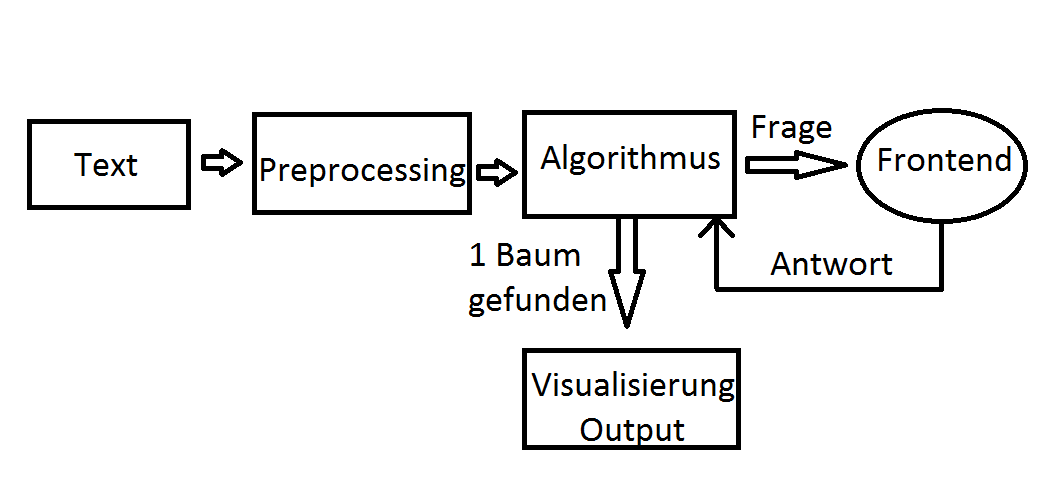
\includegraphics[scale=0.4]{Grafik}
    \begin{itemize}
        \item Generiere aus Parseforest die Frage, welche bei ihrer Beantwortung die meisten Bäume rausfiltert.
            \begin{itemize}
                    \vspace{5pt}
                \item Suche des Tupels, das den Suchraum am ehesten halbiert:
            \end{itemize}
    \end{itemize}
    \vspace{5pt}

        a $\gets$ len(parses) Anzahl der Parse-Bäume. \\
        For each tuple \\
        score $\gets$ $\mathrm{abs}(\mathrm{count(tuple)} - \frac{a}{2})$ \\
        End For

    \vspace{5pt}
    \begin{itemize}
        \item Nimm den Tupel als Frage
    \end{itemize}


\subsubsection{Dependencies}
\label{ssub:Server-Dependencies}

    \begin{itemize}
            \vspace{10pt}
        \item Python 3.4 oder neuer (aufgrund des Pakets \texttt{asyncio})
            \vspace{10pt}
        \item Parser, der k-best Parses liefert
            \vspace{10pt}
        \item TCP- oder UNIX-Sockets
        	\vspace{10pt}
        \item JSON
    \end{itemize}

\subsubsection{Algorithm}
\label{ssub:Algorithm}

\subsection{AaS-CLI-Client}
\label{sub:AaS-CLI-Client}

\subsubsection{Dependencies}
\label{ssub:CLI-Client-Dependencies}

\subsection{AaS-Web-Client}
\label{sub:AaS-Web-Client}

\subsubsection{Dependencies}
\label{ssub:Web-Client-Dependencies}

\end{document}
